\Exhibit{FlutterContributions}{%
    Скриншоты пакетов Flutter, где Алексей Инкин был неглавным контрибьютором%
}

Для каждого пакета приведены два скриншота.
Первый -- страница пакета на pub.dev, подтверждающая метрику популярности
и адрес репозитория GitHub с исходным кодом пакета,
чтобы сопоставить его со вторым скриншотом.
Обратите внимание, что курсор наведён на ссылку `Repository (GitHub)',
так что адрес репозитория показывается слева внизу.

Второй скриншот -- контрибьюторы в код пакета на GitHub.

1. Пакет `visibility\_detector', автор -- Google, популярнее 99\% пакетов Dart:

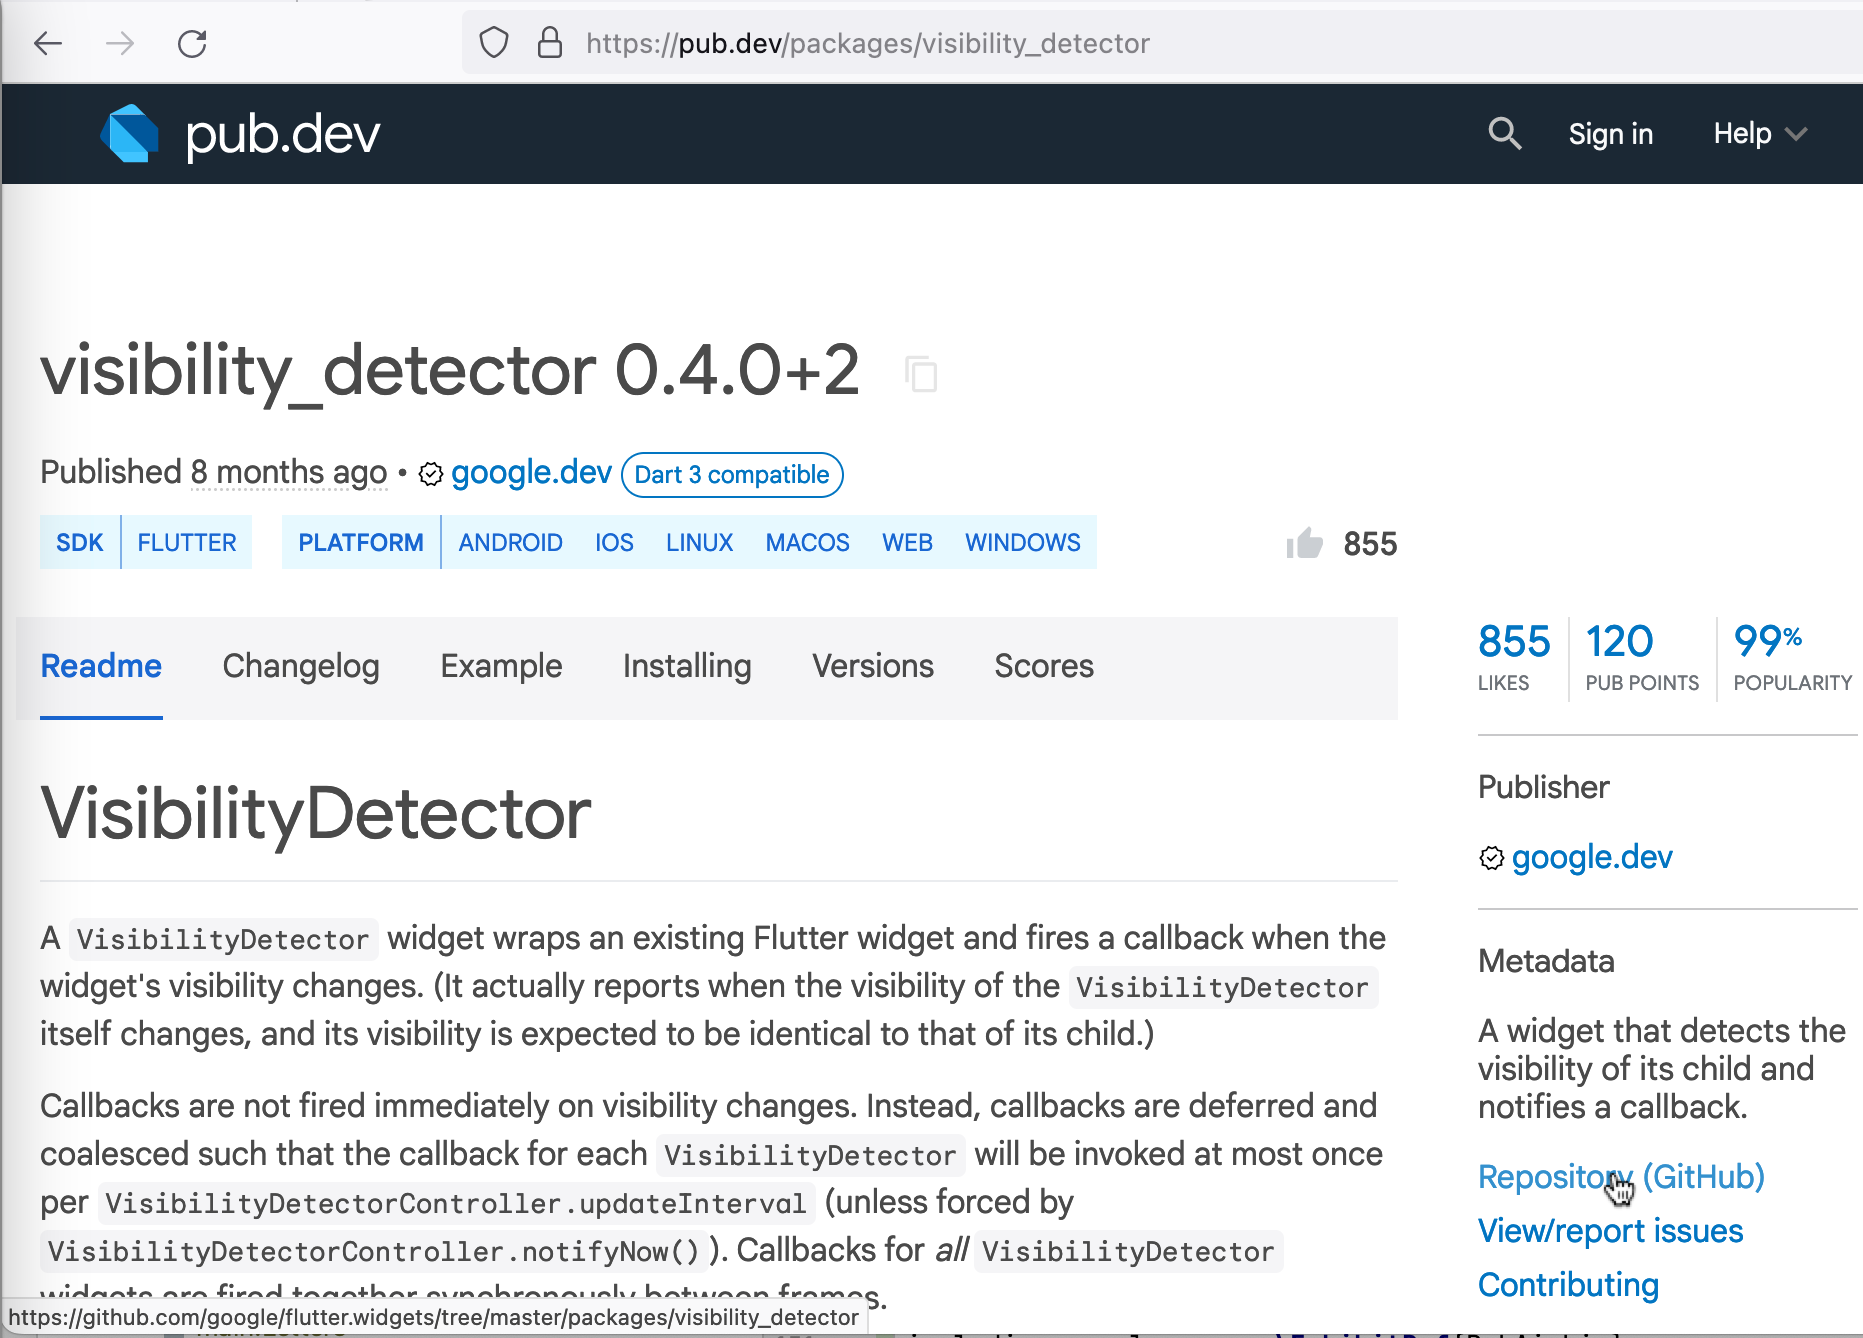
\includegraphics[width=\textwidth]{visibility_detector}
\pagebreak

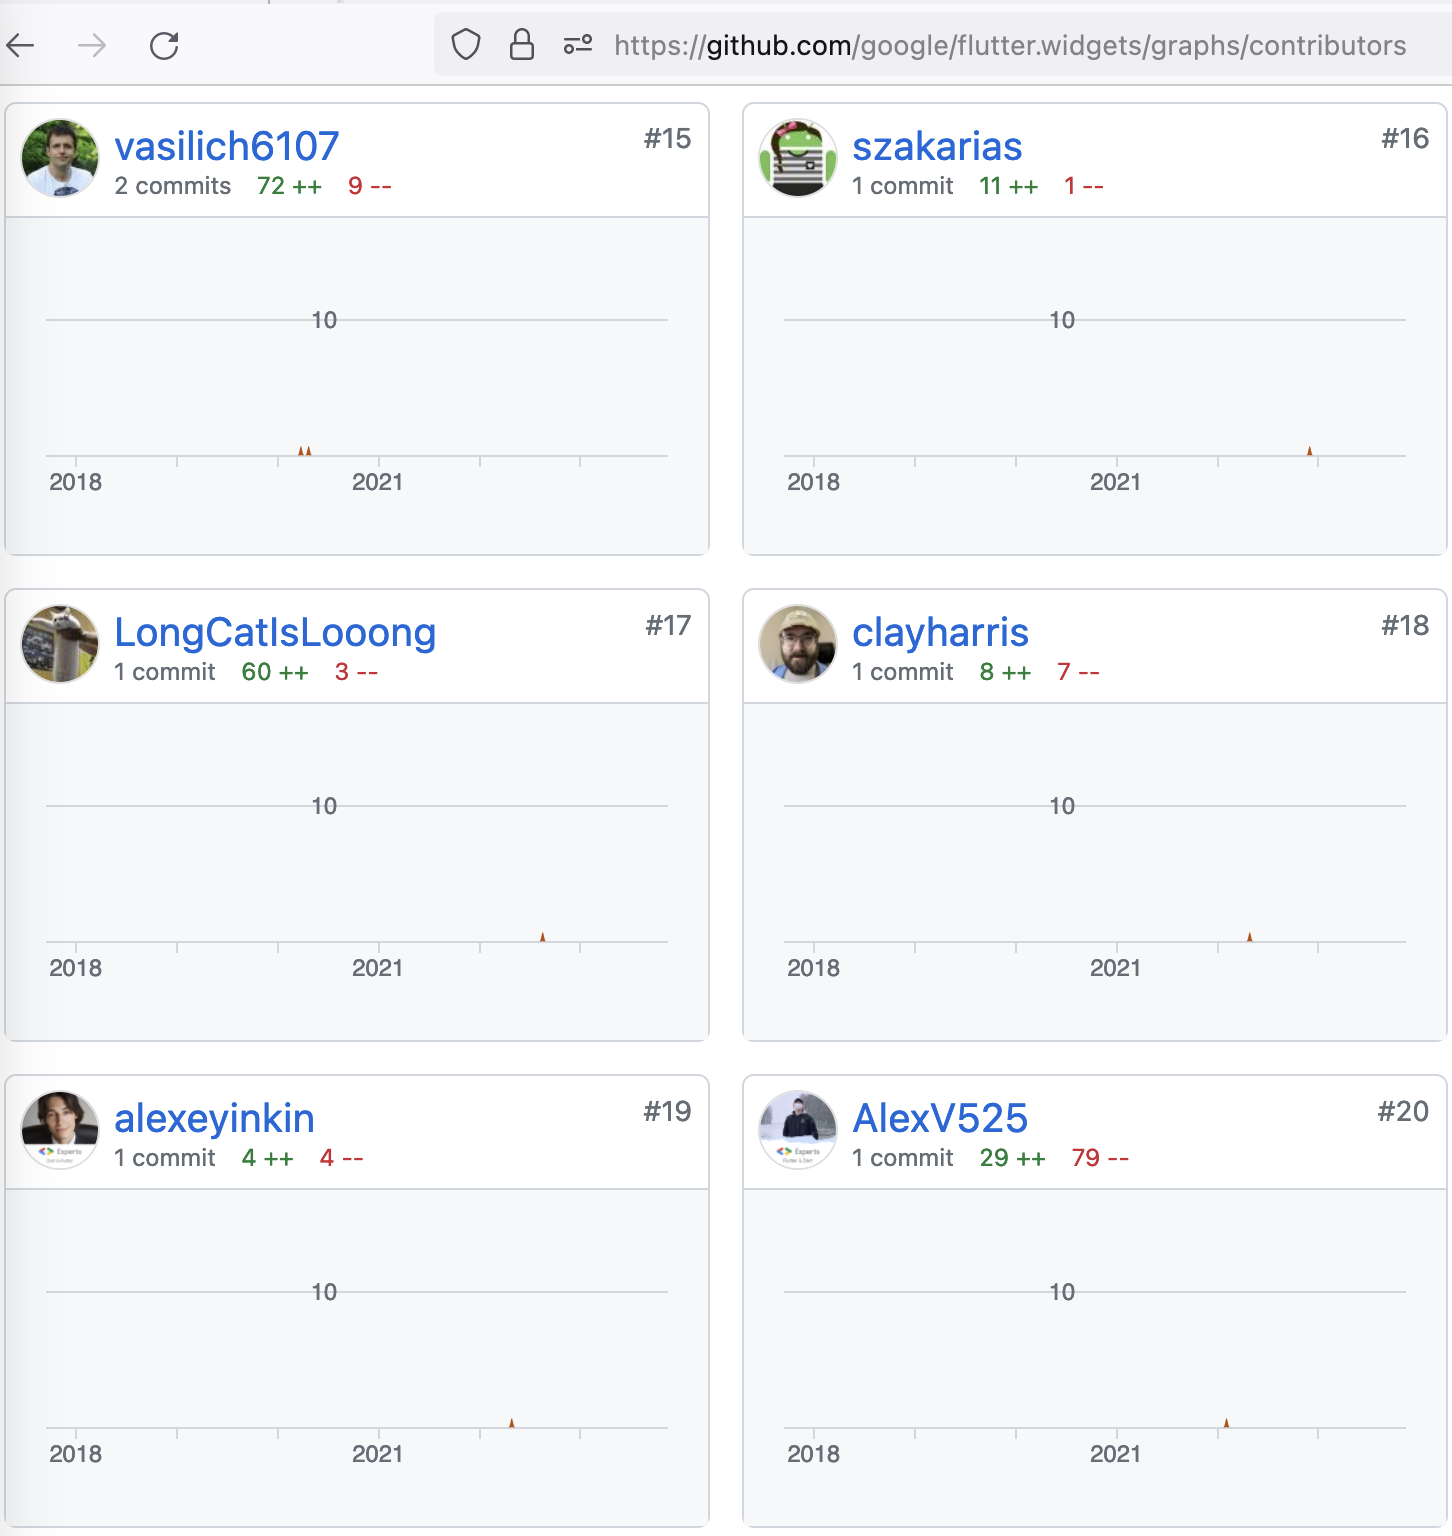
\includegraphics[width=\textwidth]{visibility_detector_contributors}
\pagebreak

2. Пакет `easy\_localization\_loader', популярнее 96\% пакетов Dart:

\begin{center}
    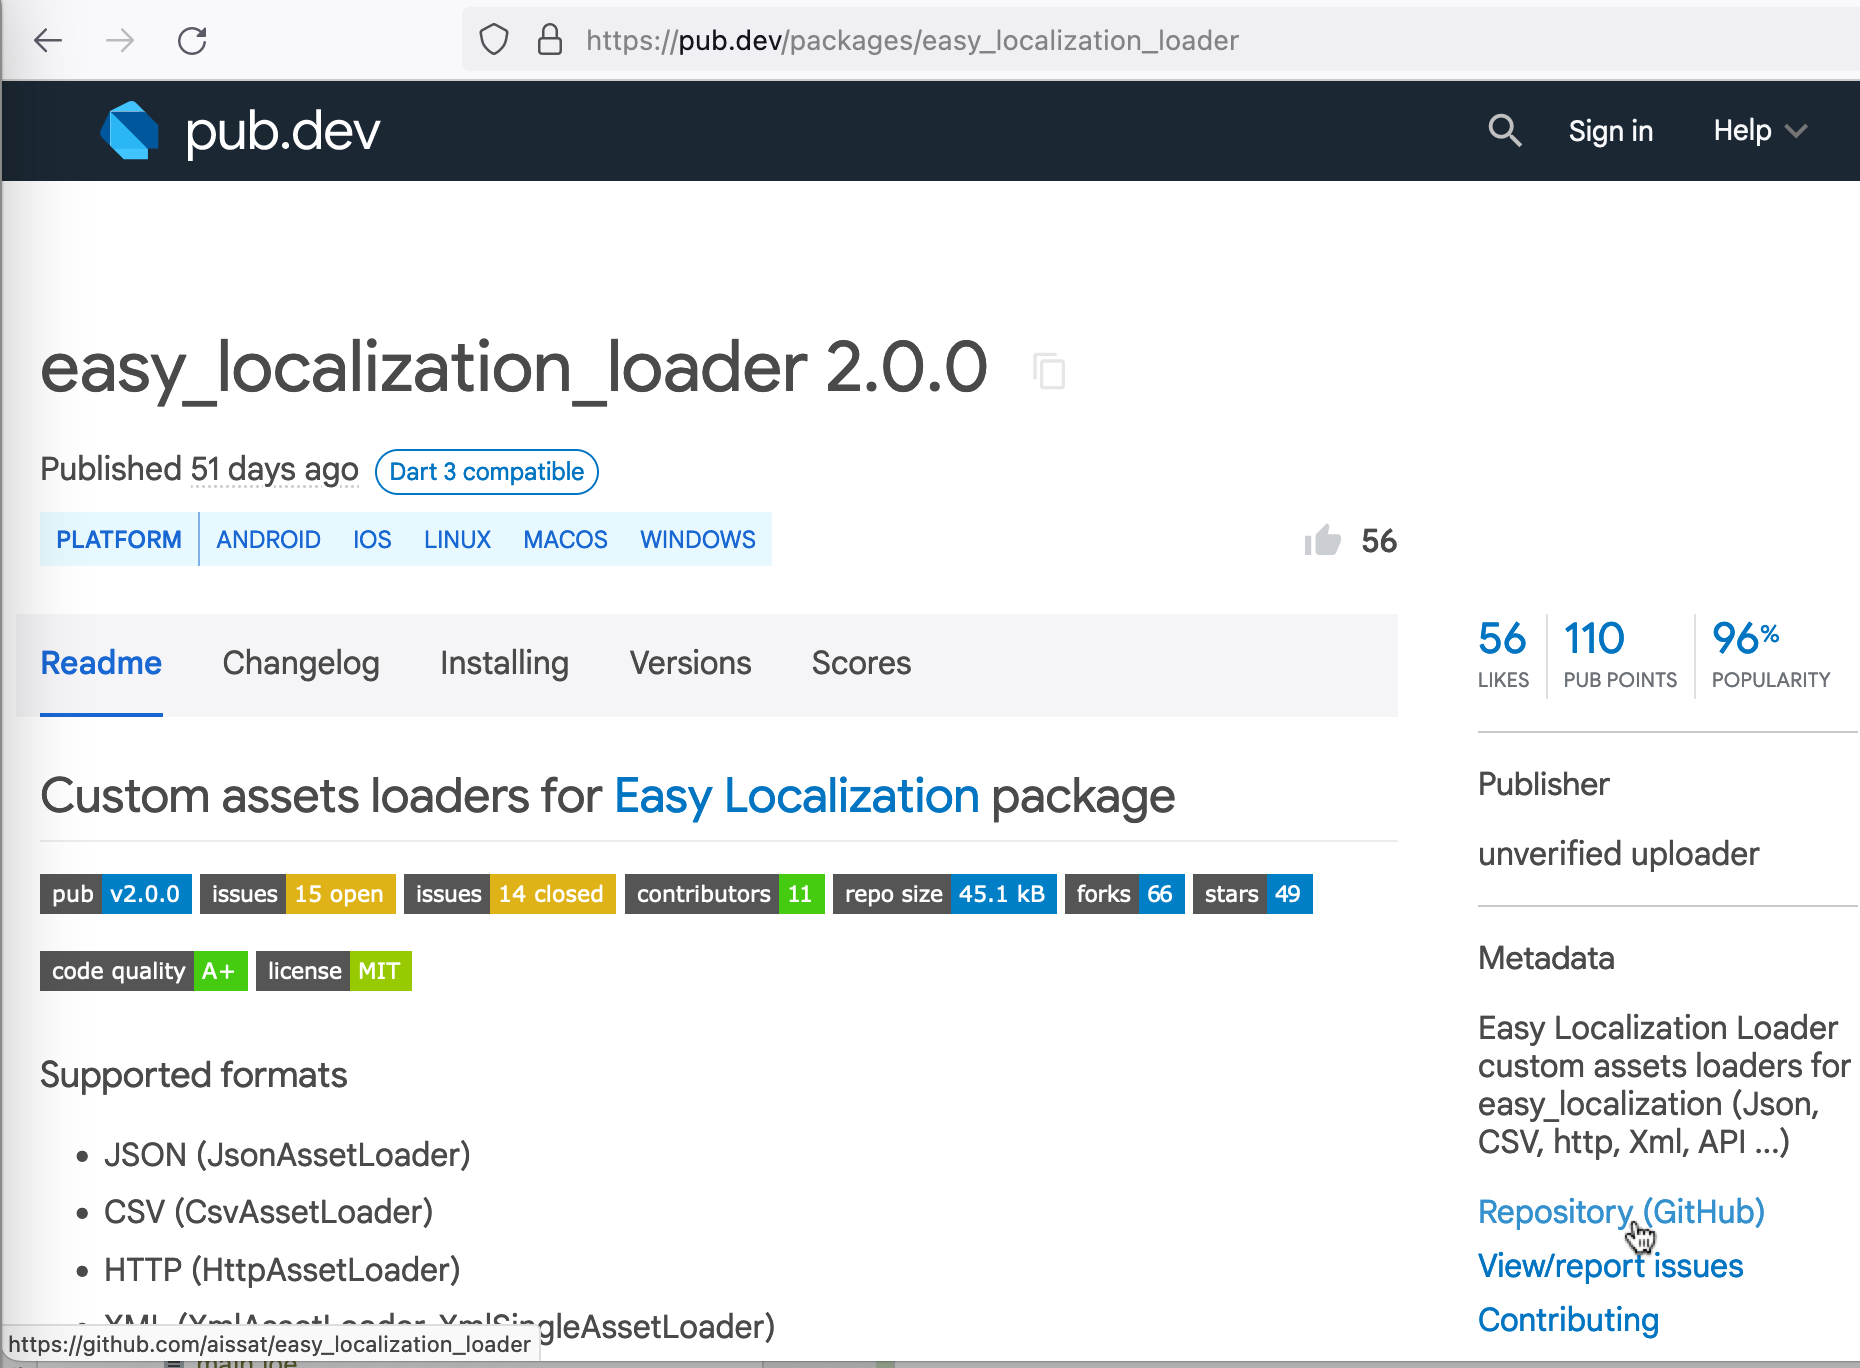
\includegraphics[width=\textwidth]{easy_localization_loader}
\end{center}
\begin{center}
    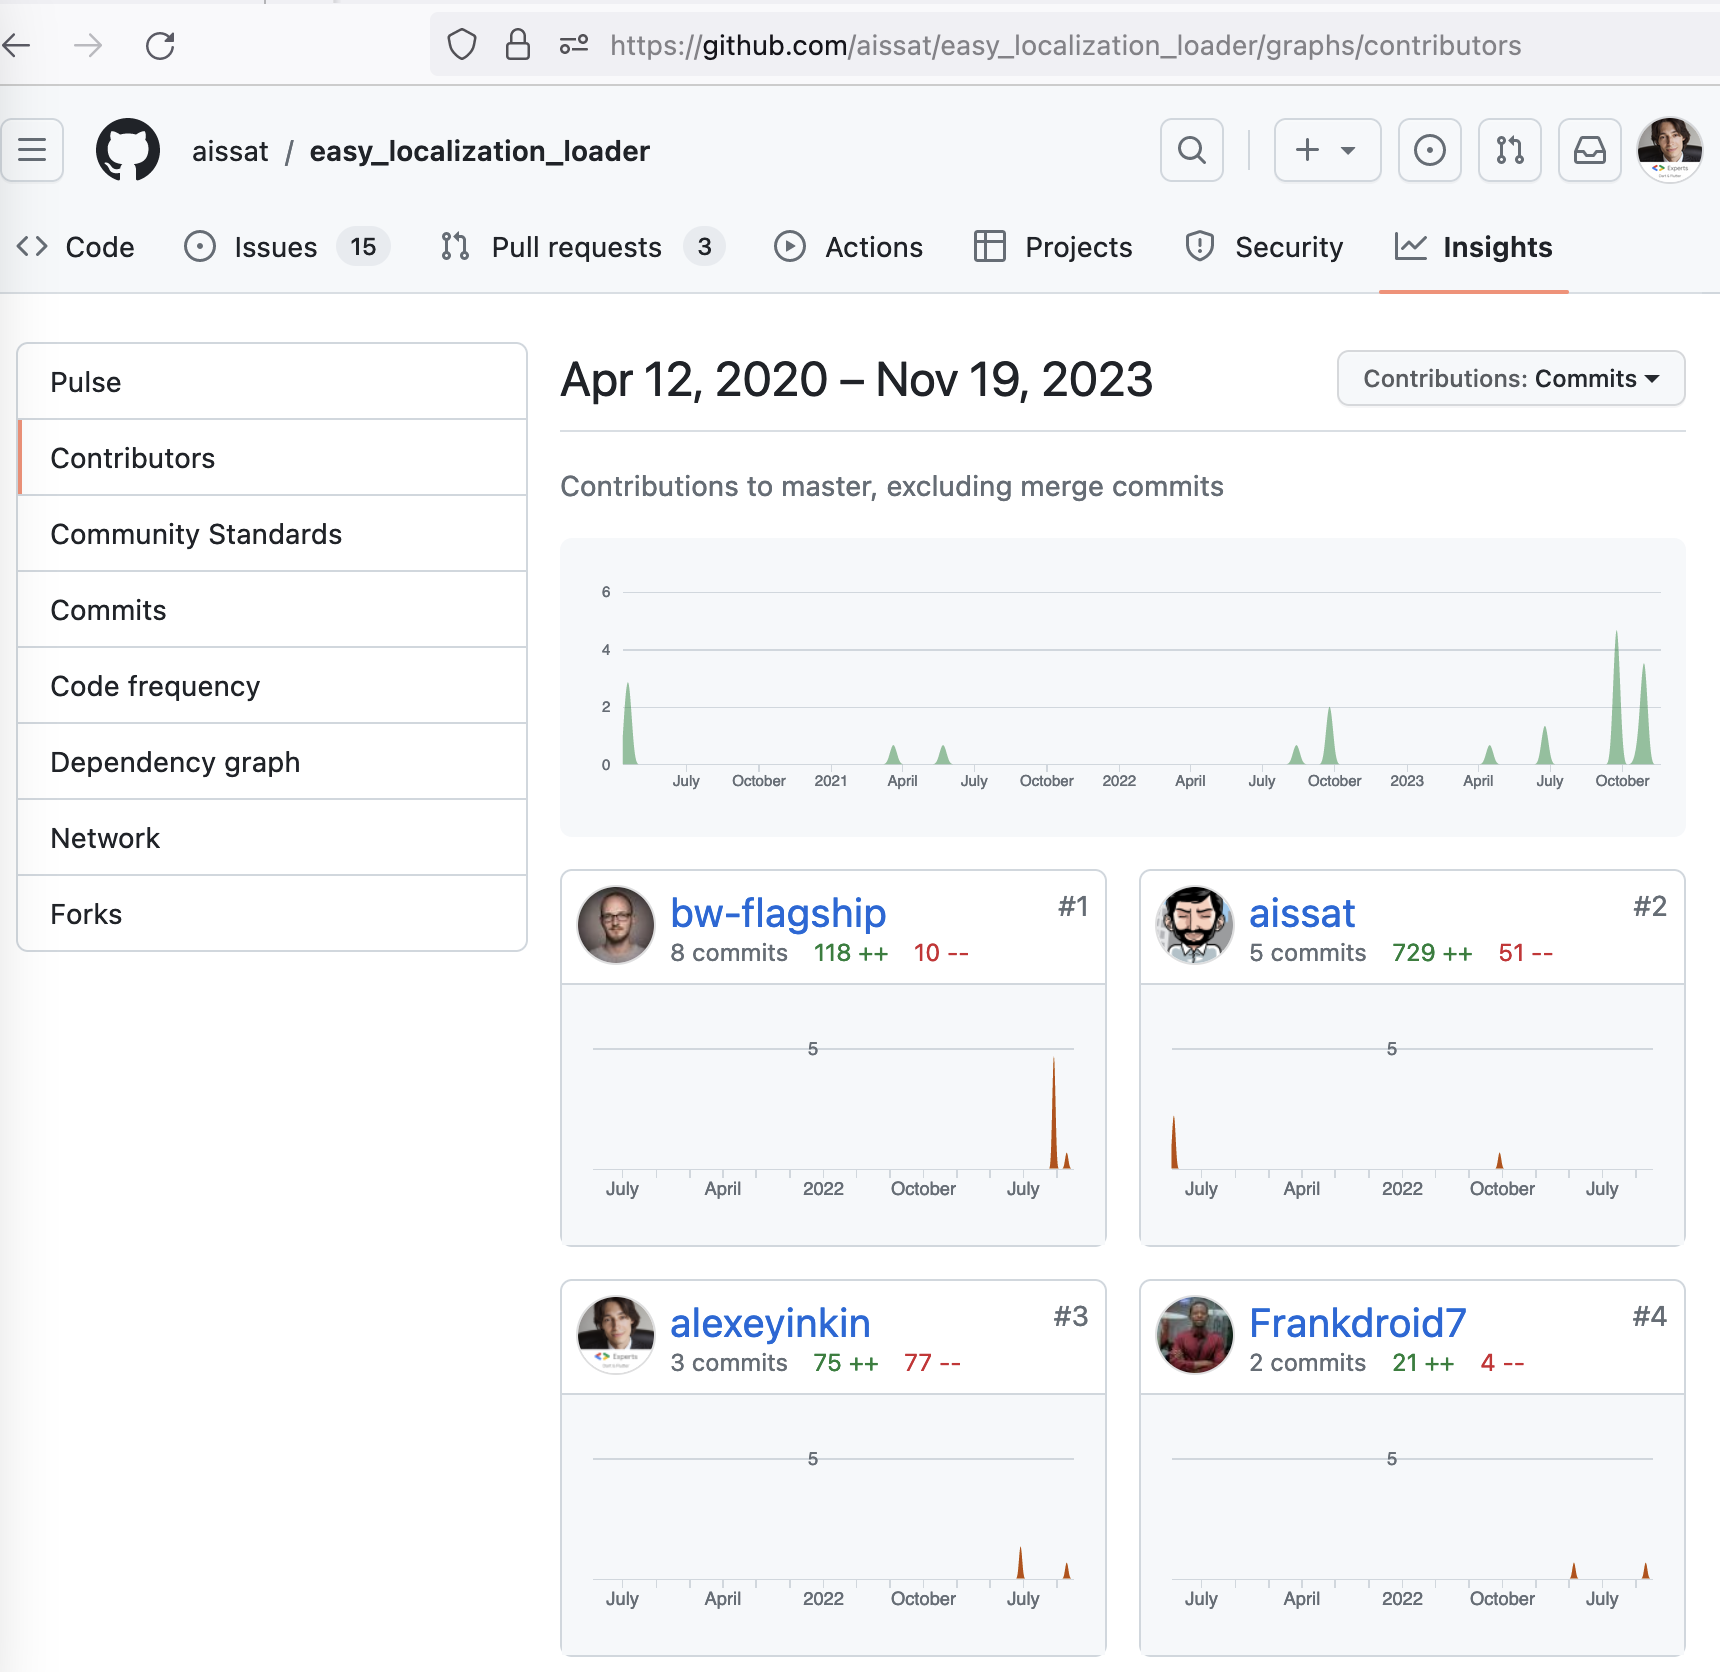
\includegraphics[width=\textwidth]{easy_localization_loader_contributors}
\end{center}
\pagebreak

3. Пакет `web3dart', популярнее 96\% пакетов Dart:

\begin{center}
    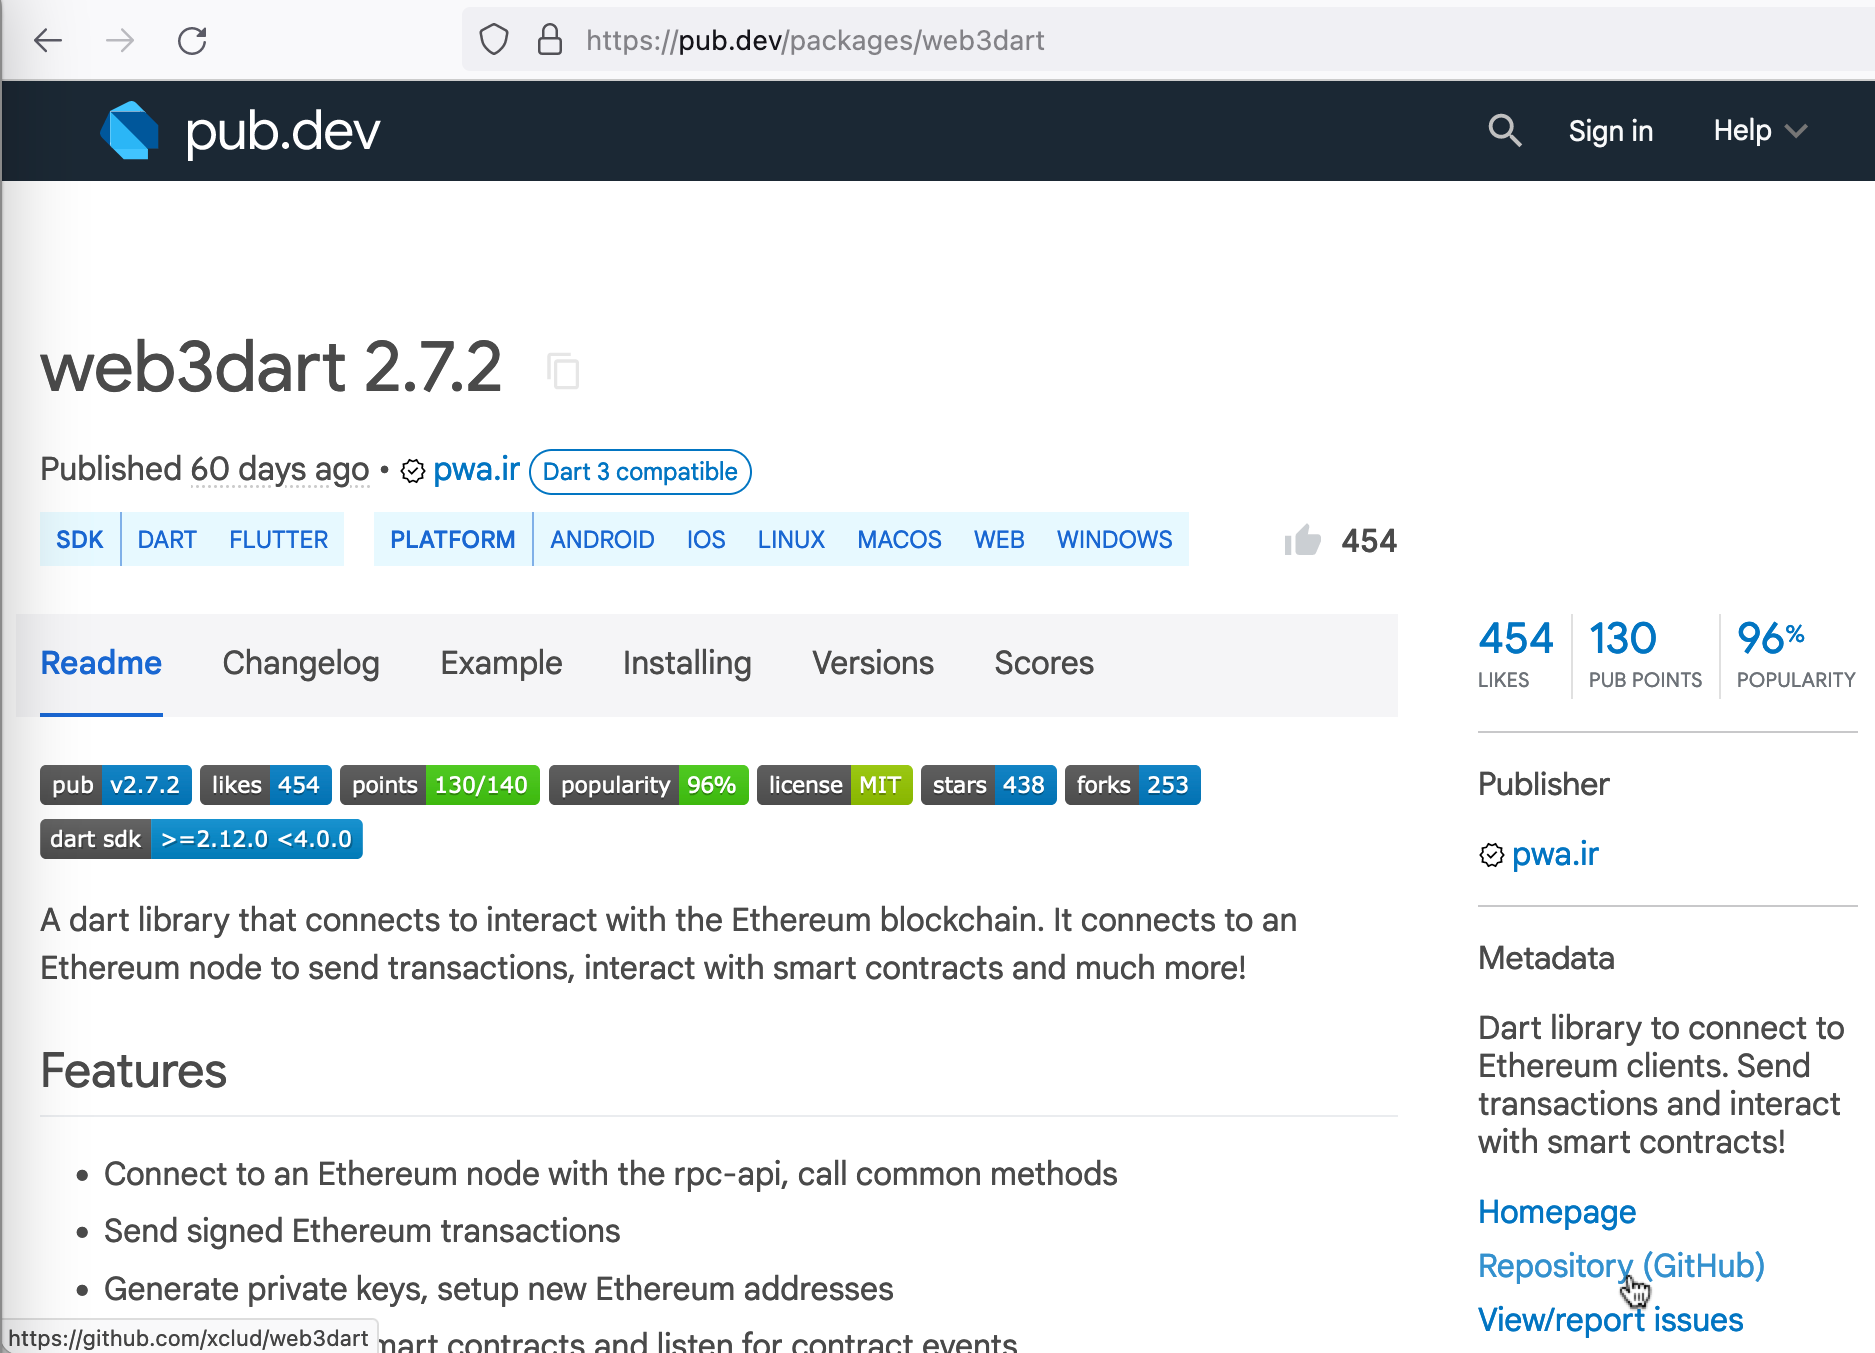
\includegraphics[width=\textwidth]{web3dart}
\end{center}
\begin{center}
    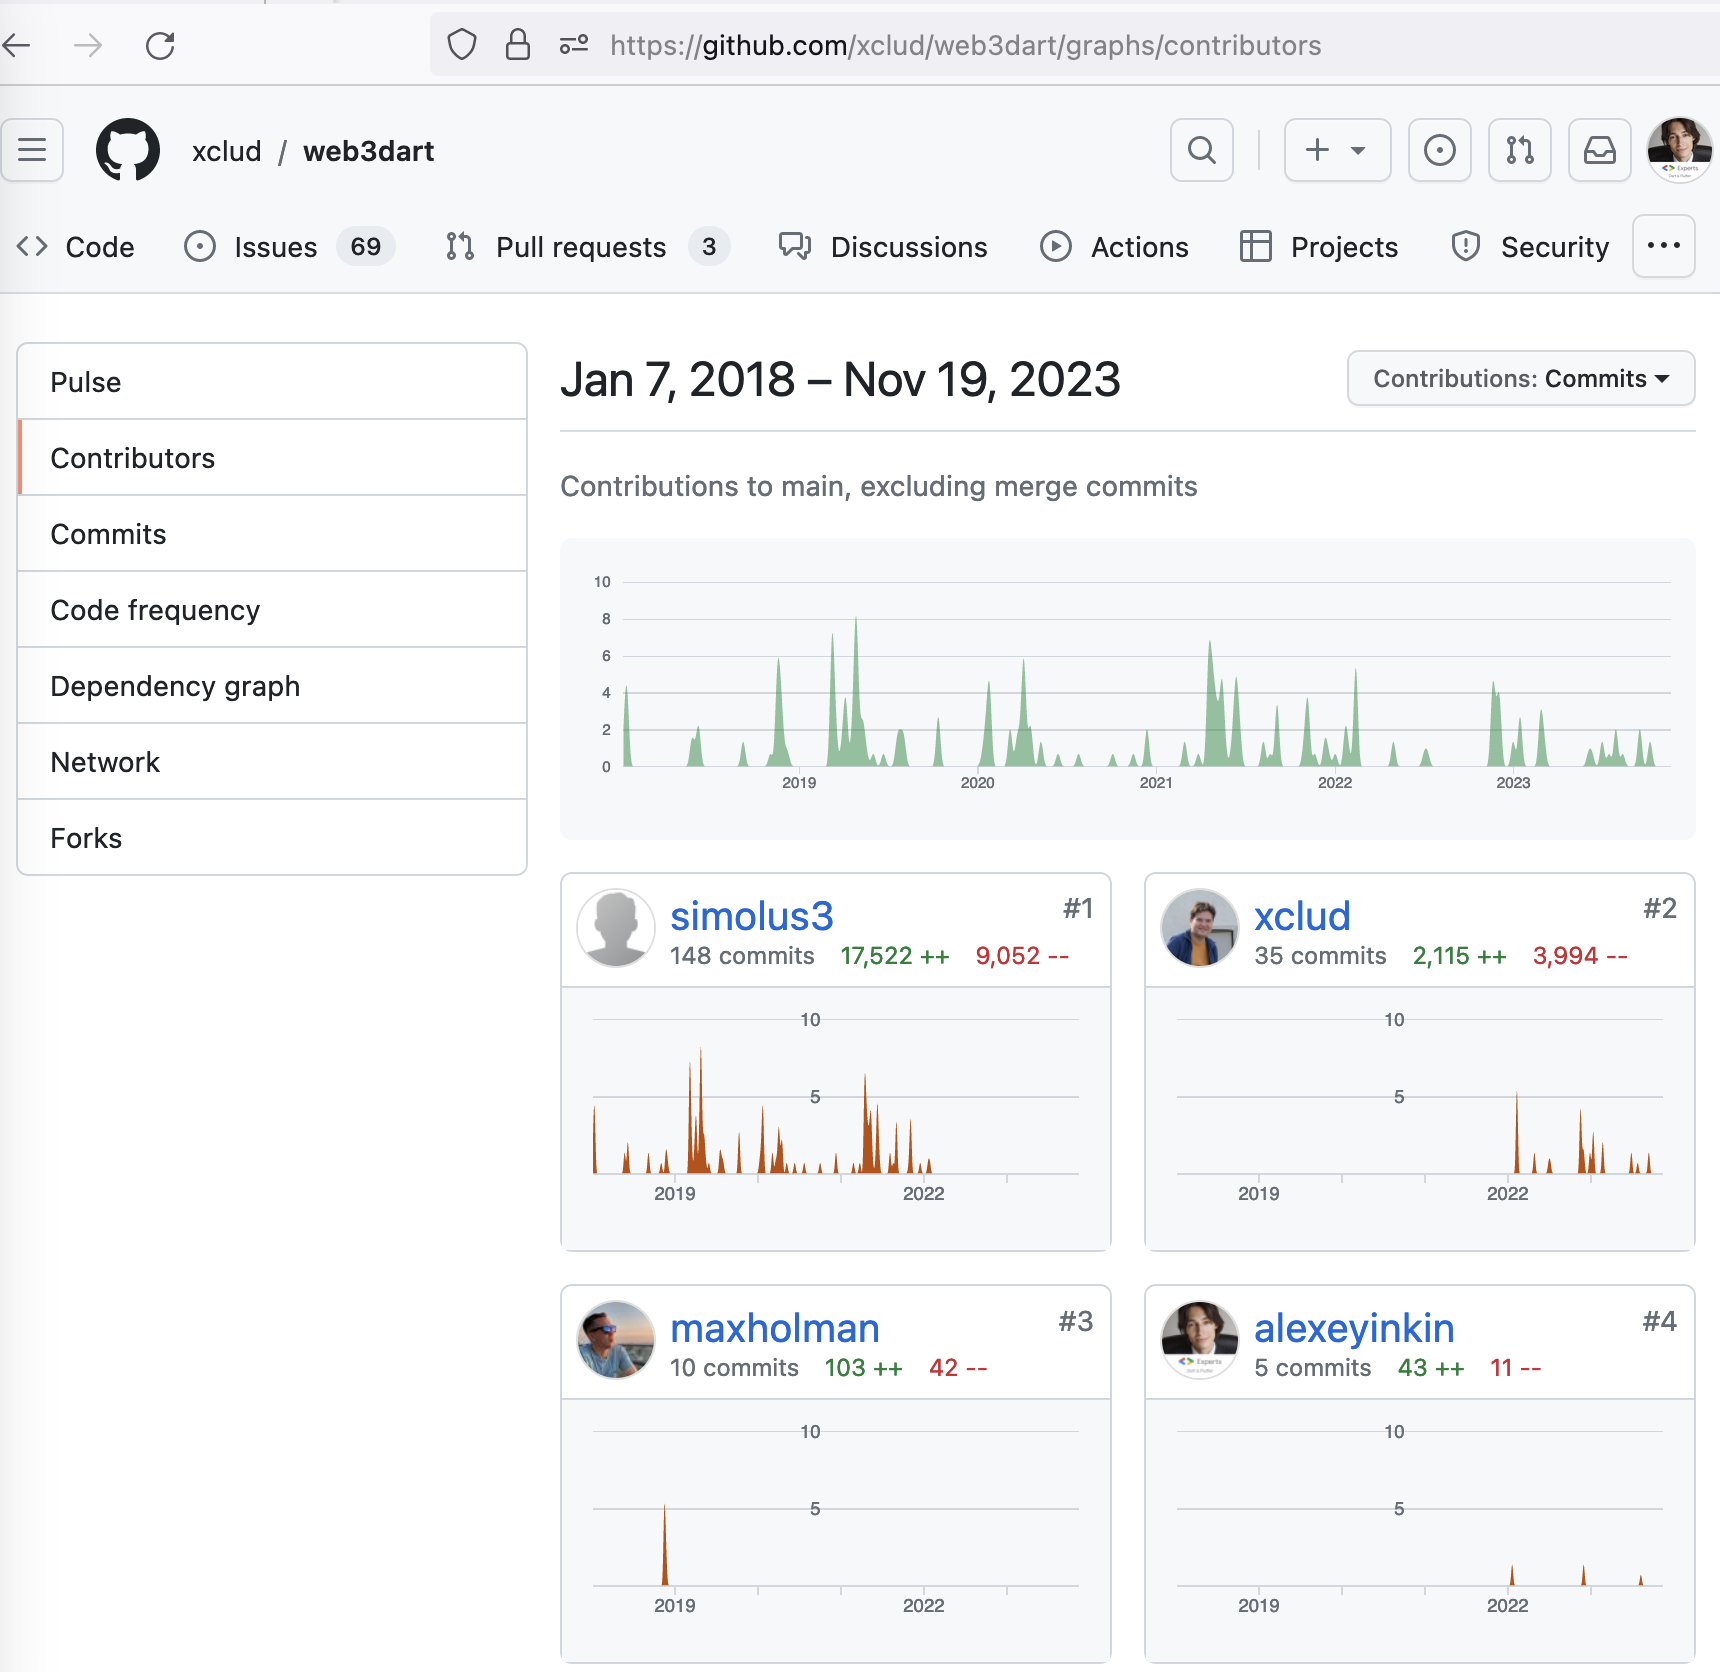
\includegraphics[width=\textwidth]{web3dart_contributors}
\end{center}
\pagebreak

\pagebreak
